% ----------------------------------------------------------------------
% Packages
% ----------------------------------------------------------------------
\usepackage[T1]{fontenc}
\usepackage{babel,booktabs,csquotes,lmodern,tikz,verbatim}
% ----------------------------------------------------------------------

\usetikzlibrary{shapes}

% ----------------------------------------------------------------------
% New commands for this document
% ----------------------------------------------------------------------
\newcommand*{\BibTeX}{BibTeX}
\newcommand*{\cls}[1]{\textsf{#1}}
\newcommand*{\cs}[1]{\texttt{\char`\\#1}}
\newcommand*{\marg}[1]{\texttt{\char`\{#1\char`\}}}
\newcommand*{\meta}[1]{\ensuremath{\langle}\emph{#1}\ensuremath{\rangle}}
\newcommand*{\oarg}[1]{\texttt{[#1]}}
\newcommand*{\pkg}[1]{\textsf{#1}}

\providecommand*{\slidesonly}[1]{#1}

\AtBeginDocument
  {
    \renewcommand*{\LaTeX}{LaTeX}
    \renewcommand*{\LaTeXe}{LaTeX2e}
    \renewcommand*{\TeX}{TeX}
  }
% ----------------------------------------------------------------------

% ----------------------------------------------------------------------
% Meta-data
% ----------------------------------------------------------------------
\title{\LaTeX{} Training Course}
\subtitle{\enquote{Using \LaTeX{} to write a thesis}}
\date{}
\author{UK-TUG Volunteers}
% ----------------------------------------------------------------------

\begin{document}

\begin{frame}
  \titlepage
\end{frame}

\maketitle

\tutornote{Time: 10:15}

\tableofcontents

\mode<presentation>%
  {
    \begin{frame}{Outline}
      \tableofcontents
    \end{frame}
  }

\section{An overview of \LaTeX{}}

\begin{frame}{\LaTeX{} is a powerful system}

  \begin{itemize}
    \item \LaTeX{} can be used from a one page letter to a 1000~page
      textbook;
    \item Most of \emph{our} examples will be simple;
    \item Complex documents, for example interactive books and
      these slides, use the same ideas as we'll explore today;
    \item By separating input from output, reusing material becomes 
      much easier.
  \end{itemize}
  
\end{frame}

\tutornote{Demo documents here}

\begin{frame}{What is \LaTeX{}, and what is \TeX{}?}

  \begin{itemize}
    \item \TeX{} is a typesetting application;
    \item \TeX{} uses \emph{primitives} to determine how to put text
      on a page;
    \item For most practical purposes, we need a \emph{format} built 
      on top of \TeX{}, for example:
      \begin{itemize}
        \item Plain \TeX{};
        \item \LaTeX{};
        \item Con\TeX{}t;
      \end{itemize}
    \item You can think of \LaTeX{} as an interpreter between you and
      \TeX{}.
  \end{itemize}

\end{frame}

\begin{frame}{\TeX{} \enquote{engines}}

  \begin{block}{pdf\TeX{}}
    The standard binary program: we'll be using this today.
  \end{block}
  
  \begin{block}{Xe\TeX{}}
    A merger of \TeX{} with modern font technology with support
    for native Unicode input and bidirectional typesetting.
  \end{block}
  
  \begin{block}{Lua\TeX{}}
    Also a modern engine: integrates the Lua scripting into \TeX{}.
  \end{block}
  
\end{frame}

\begin{frame}{What do we need to use \LaTeX{}?}

  \begin{itemize}
    \item A \TeX{} distribution: \TeX{} Live (Windows, Mac, Linux) or
      MiK\TeX{} (Windows only);
    \item A text editor, \emph{e.g.}~Notepad, TextEdit, Emacs;
    \item A PDF viewer, for example Adobe Reader.
  \end{itemize}

  \pause
  
  Usually, we use a specialist editor
  \begin{itemize}
    \item Coloured syntax;
    \item Buttons or menus to run \LaTeX{}, \emph{etc.};
    \item Most include an integrated spell checker.
  \end{itemize}
\end{frame}

\tutornote{Time: 10:30}

\section{Getting started}

\begin{frame}{\LaTeX{} is not a word processor}

  \begin{itemize}
    \item \LaTeX{} input is stored as plain text files, usually with
      the extension \texttt{.tex};
    \item \LaTeX{} input files contain both the text of the document
      and \emph{commands};
    \item Commands start with a slash, so look like this:
      \cs{example};
    \item Writing in \LaTeX{} is therefore a bit like \emph{programming}
      it to produce the document you want;
    \item \emph{Logical} mark up is important in \LaTeX{}: we'll use some
      almost straight away!
  \end{itemize}

\end{frame}

\begin{frame}{Workflow}

  \resizebox{\linewidth}{!}{%
    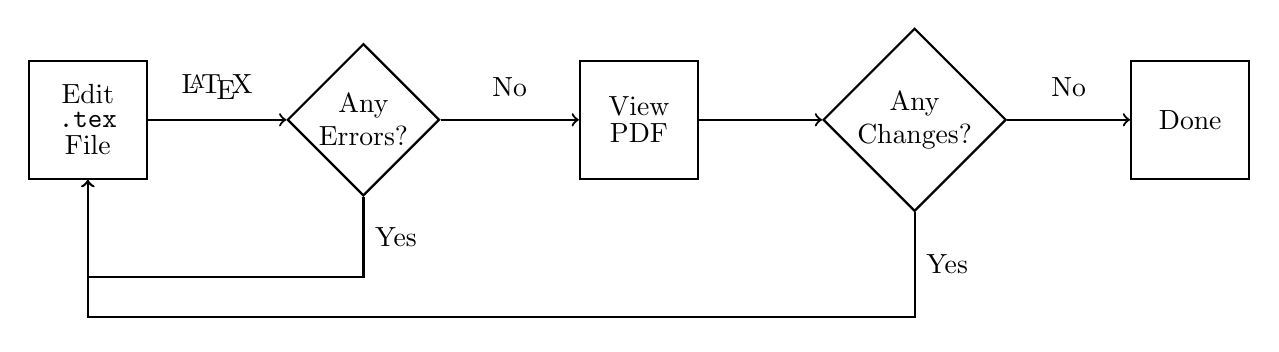
\begin{tikzpicture}[
      minimum width  = 1.5 cm,
      minimum height = 1.5 cm,
      inner sep      = 0.1 em,
      thick
    ]
      \path (0,0) node[draw] (edit) {\shortstack{Edit\\\texttt{.tex}\\File}} ;
      \path (3.5,0) node[draw,diamond] (errors) 
        {\shortstack{Any\\Errors?}};
      \path (7,0) node[draw] (pdf) {\shortstack{View\\PDF}};
      \path (10.5,0) node[draw,diamond] (change) 
        {\shortstack{Any\\Changes?}};
      \path (14,0) node[draw] (done) {Done};
      \draw[->] (edit) -- (errors) node[midway,above=-1em] 
        {\LaTeX{}};
      \draw[->] (errors) -- ++(0,-2) node[midway,right=-1em] 
        {Yes} -| (edit);
      \draw[->] (errors) -- (pdf) node[midway,above=-1em] {No};
      \draw[->] (pdf) -- (change);
      \draw[->] (change) -- ++(0,-2.5) node[midway,right=-1em] 
        {Yes} -| (edit);
      \draw[->] (change) -- (done) node[midway,above=-1em] {No};
    \end{tikzpicture}
  }
  
\end{frame}

\begin{frame}[fragile]{Spacing}

  \begin{itemize}
    \item \LaTeX{} treats multiple spaces as a single space;
    \item By default, the space between sentences is slightly larger
      than the space between words -- can be switched off using
      \cs{frenchspacing};
    \item The tilde (\verb|~|) is used to create a non-breaking space;
    \item New line characters are treated as a space;
    \item Paragraph breaks should be indicated by a blank line;
    \item \LaTeX{} automatically indents paragraphs, except for the
      first paragraph after a section heading.
  \end{itemize}
  
\end{frame}

\begin{frame}[fragile]{A simple document}
  \begin{block}{Example}
    \begin{semiverbatim}
\alert<2>{\\documentclass}\alert<2,4>{[a4paper,12pt]}\alert<2-3>{\{article\}}
\alert<5>{\% A comment in the preamble}
\alert<6>{\\begin\{document\}}
\alert<7>{\% This is a comment}
\alert<8>{This is   a simple}
\alert<8>{document\\footnote\{with a footnote\}.}

\alert<8>{This is a new paragraph.}
\alert<6>{\\end\{document\}}
    \end{semiverbatim}
  \end{block}
  
\end{frame}

\tutornote{Show demo document in \TeX{}works, and mention Sync\TeX{}}

\begin{exercise}
  Use the editor of your choice to create the above document. While you
  can use a specialist editor, start by doing this example in a basic
  editor such as Notepad. Save the document with a \texttt{.tex}
  extension, for example \texttt{exercise1.tex}, then go to a
  Terminal/Command Prompt and type:
  \begin{verbatim}
    pdflatex exercise1
  \end{verbatim}
  You can then view the resulting PDF file using a PDF viewer such as
  Adobe Reader.
  
  Try experimenting with white space: what do multiple spaces and 
  multiple lines do? Also try out using the tilde (\verb"~") for 
  a non-breaking space and \cs{,} for spaces of different
  widths.
  
  \LaTeX{} automatically indents new paragraphs: see what the \cs{noindent}
  macro does to these cases.
\end{exercise}

\tutornote{Finish exercise at 10:50}

\section{Logical structure}

\begin{frame}[fragile]{Logical mark up}

  \LaTeX{} provides us with logical mark up, as well as the ability to
  directly set the appearance. 
  \begin{block}{Logical mark up}
      \cs{emph}\marg{\meta{text}}\\
      \marg{\cs{large} \meta{text}}
  \end{block}
  \begin{block}{Appearance mark up}
      \cs{textit}\marg{\meta{text}}\\
      \marg{\cs{fontsize}\marg{12 pt}\marg{14 pt}\cs{selectfont} \meta{text}}
  \end{block}
  Usually, logical mark up is best when it is available.

\end{frame}

\begin{frame}{Title Page}

  First, you need to give the \enquote{meta-data}:
  \begin{itemize}
    \item \cs{title}\marg{\meta{title}}
    \item \cs{author}\marg{\meta{author(s)}}
    \item \cs{date}\marg{\meta{date}} (optional)
  \end{itemize}
   Then use \cs{maketitle} to display the title page.
   
\end{frame}

\begin{frame}{Sectioning commands}

  \begin{itemize}
    \item 
      \alert<2>{\cs{chapter}\oarg{\meta{short title}}\marg{\meta{title}}}
    \item \cs{section}\oarg{\meta{short title}}\marg{\meta{title}}
    \item \cs{subsection}\oarg{\meta{short title}}\marg{\meta{title}}
    \item \cs{subsubsection}\oarg{\meta{short title}}\marg{\meta{title}}
    \item 
      \alert<3>{\cs{paragraph}\oarg{\meta{short title}}\marg{\meta{title}}}
    \item \cs{subparagraph}\oarg{\meta{short title}}\marg{\meta{title}}
  \end{itemize}
  
\end{frame}

\begin{exercise}
  Try producing the following document.
  \verbatiminput{examples/example2}
  
  Experiment with the logical mark up for appearance, for example
  \cs{emph}, \cs{large}, \cs{Large} and \cs{Huge}. Compare these
  with the direct changes brought about by \cs{textit} and \cs{textbf}.
  
  Try changing the format of text for a longer block by trapping the
  formatting changes within \cs{begingroup} and \cs{endgroup}, for
  example
  \begin{verbatim}
    \begingroup
      \large
      \itshape
      Some text
      
      A second paragraph
    \endgroup
  \end{verbatim}
  
\end{exercise}

\begin{frame}[fragile]{Lists}

  \begin{block}{Order not important}
\begin{verbatim}
  \begin{itemize}
    \item This is an unordered list
  \end{itemize}
\end{verbatim}
  \end{block}
  
  \begin{block}{Order important}
\begin{verbatim}
  \begin{enumerate}
    \item This one is ordered
    \item So this will have number 2!
  \end{enumerate}
\end{verbatim}
  \end{block}

\end{frame}

\begin{exercise}
  Make some lists, and nest one list inside another. How does the
  format of the numbers or markers change? You can only go to
  four levels with standard \LaTeX{}, but more than four nestings
  tends to be a bad sign anyway!
\end{exercise}

\tutornote{Finish exercise at 11:30}

\section{Classes}

\begin{frame}{Document classes}

  The \emph{document class} sets up the general layout of the document,
  for example:
   \begin{itemize}
     \item the format of the headings;
     \item if the document should have chapters;
     \item if the title should be on a separate page or above 
       the text on the first page;
   \end{itemize}
   They can also add new control sequences.

  \begin{block}{Usage}
      \cs{documentclass}\oarg{\meta{options}}\marg{\meta{class-name}}
  \end{block}
\end{frame}

\begin{frame}{Base classes}

  \begin{description}
    \item[\cls{article}] for short documents without chapters;
    \item[\cls{report}] for longer documents with chapters,
      typically single-sided with an abstract;
    \item[\cls{book}] for books, typically double-sided with
      front matter and back matter;
    \item<2->[\cls{letter}] for correspondence;
    \item<2->[\cls{slides}] for presentations.
  \end{description}

\end{frame}

\begin{frame}{Modern classes}

  \begin{description}
    \item[\cls{KOMA-Script}] \cls{scrartcl}, \cls{scrreprt}
      and \cls{scrbook} to replace \cls{article}, \cls{report}
      and \cls{book}, respectively;
    \item[\cls{memoir}] replaces \cls{book} and \cls{report};
    \item[\cls{beamer}] for slides (used to create the course 
      material).
  \end{description}
  
\end{frame}

\begin{frame}[fragile]{KOMA-Script Example}

  \verbatiminput{examples/example3}

\end{frame}

\begin{frame}{Documentation}

  \begin{block}{On your computer}
    The \texttt{texdoc} application will show documentation for 
    material you have installed. From the Command Prompt/Terminal
    \begin{center}
      \texttt{texdoc \meta{name}}
    \end{center}
  \end{block}
  
  \begin{block}{From CTAN}
    Try the web address
    \begin{center}
      \texttt{http://ctan.org/pkg/\meta{name}}
    \end{center}
  \end{block}

\end{frame}

\begin{exercise}
  Try creating the above document. The KOMA-Script classes have
  various options that affect the document's appearance. Try
  experimenting with some of the following: \texttt{chapterprefix}, 
  \texttt{headings=small}, \texttt{headings=normal},
  \texttt{headings=big}, \texttt{numbers=enddot},
  \texttt{numbers=noenddot}.  For example:
  \begin{verbatim}
    \documentclass[chapterprefix]{scrreprt}
  \end{verbatim}
  
  Also try making simple documents with \textsf{memoir}:
  see how without any other changes the appearance of the PDF
  file is altered.
  
  To add some \enquote{dummy text} to your files, put the line
  \verb"\usepackage{lipsum}" before \verb"\begin{document}", then
  put \cs{lipsum} somewhere after \verb"\begin{document}". This 
  will create a number of filler paragraphs. Use this to see what effect
  the \texttt{twocolumn} class option has on the layouts you see.
  
  Use \textsf{texdoc} to look up the documentation for the classes
  we are using. Some of these are very long: most of the time you only
  need a small subset of the commands available!
\end{exercise}

\section{Cross-referencing}

\begin{frame}[fragile]{Cross-referencing}

  \begin{block}{Example input}
    \begin{verbatim}
\section{A section}
\label{sec:interesting}
...
\ref{sec:interesting}
    \end{verbatim}
  \end{block}
  
  \emph{Two} \LaTeX{} runs are needed to get cross-references right.

\end{frame}

\tutornote{Mention \textsf{cleveref}}

\begin{exercise}
  Try producing the following document.
  \verbatiminput{examples/example4}
  
  Experiment with cross-references to sections, subsections and items in
  ordered lists. Can you see who it works?
\end{exercise}

\tutornote{Finish exercise at 12:30 and go to lunch. Restart at 13:15.}

\section{More logical structure}

\begin{frame}[fragile]{Mathematics}

  \begin{itemize}
    \item Mathematical content is marked up in \LaTeX{} in a logical way;
    \item You can use \$ \ldots \$ or \cs{(} \ldots \cs{)} to mark up
      in-line maths;
    \item For displayed mathematics, use \cs{[} \ldots \cs{]};
    \item A lot of spacing is automatic in math mode;
    \item Maths is an entire area on its own!
  \end{itemize}
  
  \begin{block}{Example input}
    \verb"\( y = 2 \sin \theta^2 \)" 
  \end{block}
  
  \begin{block}{Example output}
    \( y = 2 \sin \theta^2 \)
  \end{block}

\end{frame}

\tutornote{Mention AMS material and Vo{\ss}'s \emph{Math Mode}}

\begin{frame}{Creating your own commands}

  \begin{block}{Syntax}
    \cs{newcommand*}\cs{\meta{name}}\marg{\meta{replacement text}}\\
    \cs{newcommand*}\cs{\meta{name}}\oarg{\meta{number}}%
      \marg{\meta{replacement text}}\\
  \end{block}
  
  \begin{block}{Examples}
    \cs{newcommand*}\cs{authorname}\marg{Joseph Wright} \\
    \cs{newcommand*}\cs{important}\oarg{1}\marg{\cs{textbf}\marg{\#1}}
  \end{block}

\end{frame}

\begin{exercise}
  Create some simple mathematical content (for example \verb"y = mx + c")
  and compare the effect of \cs{(} \ldots \cs{)} with \cs{[} \ldots \cs{]}.
  Can you work out how to get capitalised Greek letters? Can you
  guess why some Greek do not seem to work?
  
  Subscripts and superscripts in math mode are created using \verb"_"
  and \verb"^", respectively. Try these out, and think about why you
  might use \cs{textsuperscript} rather than \verb"^" in some cases.
  
  Try creating your own simple commands using \cs{newcommand}. Think of
  how to create commands using 1, 2 and 3 arguments.
\end{exercise}

\tutornote{Finish exercise at 13:45.}

\section{Floating material}

\begin{frame}[fragile]{On packages}

  The \LaTeX{} kernel is rather limited: to get around that we
  load \emph{packages}:
  \begin{semiverbatim}
\cs{usepackage}\oarg{\meta{options}}\marg{\meta{package}}
  \end{semiverbatim}
  or
  \begin{semiverbatim}
\cs{usepackage}\texttt{\{\meta{package1},\meta{package2},\ldots\}}
  \end{semiverbatim} 
  We have already seen the \pkg{lipsum} package! 
  
  \vspace{1 em}
  
  \uncover<2>{%
   Documentation for packages is available in exactly the same way
   as for classes.%
  }
  
\end{frame}

\begin{frame}[fragile]{Including external images}

  \begin{itemize}
    \item Load the \pkg{graphicx} package to include graphics;
    \item Use \cs{includegraphics} to actually place the image;
    \item Image formats: \texttt{pdf}, \texttt{png}, \texttt{jpg};
    \item File extension should be omitted.
  \end{itemize}
  
  \vspace{1 em}
  \uncover<2>{%
    Graphics can also be \enquote{drawn} in \LaTeX{} using the
    Ti\emph{k}z package:\\ a course in itself!
  }

\end{frame}

\tutornote{Perhaps include keyval interface for graphics options}

\begin{frame}[fragile]{Floating figures}

  \begin{block}{A floating figure \dots}
\begin{semiverbatim}
\\begin\{figure\}\alert<2>{[htbp]}
  \alert<3>{\\centering}
  \\includegraphics\{myimage\}
  \alert<4>{\\caption\{A Sample Figure\}}
  \alert<5>{\\label\{fig:sample\}}
\\end\{figure\}
\end{semiverbatim}
  \end{block}
  
  \begin{block}<6->{\ldots needs a cross-reference}
\begin{semiverbatim}
as is show in Figure~\alert<6>{\\ref\{fig:sample\}}
\end{semiverbatim}
  \end{block}

\end{frame}

\begin{exercise}
  Try producing the following document. (Use an image application,
  such as Paint, to produce a simple picture and save it as
  \texttt{shapes.png}.)
  \verbatiminput{examples/example5}
  Here are some more class options to try that will affect the list of
  figures: \texttt{chapteratlists}, \texttt{chapteratlists=0mm}.
\end{exercise}

\begin{frame}{Tables}

  \begin{itemize}
    \item The floating environment for a table is called \texttt{table};
    \item However, the content can be anything!
    \item Use the \texttt{tabular} environment to make tables;
    \item Load the \textsf{booktabs} package for rules.
  \end{itemize}
  
\end{frame}
  
\begin{frame}[fragile]{Tables}
  
  \begin{block}{A simple table}
\begin{semiverbatim}
\alert<2>{\\begin\{table\}}
  \alert<2>{\\centering}
  \alert<2>{\\caption\{A caption\}}
  \alert<2>{\\label\{tab:example\}}
  \alert<3>{\\begin\{tabular\}}\alert<4>{\{lcr\}}
   \alert<5>{\\toprule}
      Heading \alert<6>{&} Heading \alert<6>{&} Heading \alert<7>{\\\\}
    \alert<5>{\\midrule}
      a \alert<6>{&} b \alert<6>{&} c \alert<7>{\\\\}
      d \alert<6>{&} e \alert<6>{&} f \alert<7>{\\\\}
      \alert<8>{\\multicolumn\{3\}\{c\}\{Wide text\}} \alert<7>{\\\\}
    \alert<5>{\\bottomrule}
  \alert<3>{\\end\{tabular\}}
\alert<2>{\\end\{table\}}
\end{semiverbatim}
  \end{block}

\end{frame}

\begin{exercise}

  Use the simple table example to start experimenting with tables.
  Try out different alignments using the \texttt{l}, \texttt{c} and
  \texttt{r} column types. What happens if you have too few items
  in a table row? How about too many? Experiment with the
  \cs{multicolumn} command to span across columns.
  
\end{exercise}

\tutornote{Finish exercise at 14:45.}

\section{Bibliographies}

\begin{frame}{Creating a bibliography}

  \begin{itemize}
    \item Entries are stored in a \emph{\BibTeX{} database};
    \item Inform \LaTeX{} about it using \cs{bibliography} command;
    \item These are cited using \cs{cite} in the \LaTeX{} file;
    \item Choose a style using \cs{bibliographystyle}.
  \end{itemize}
  
\end{frame}

\begin{frame}[fragile]{Creating a bibliography}{The \LaTeX{} basics}

\begin{verbatim}
\documentclass{article}
\usepackage{natbib}
\bibliographystyle{plainnat}
\begin{document}
Some text \cite{key}.
\bibliography{example}
\end{document}
\end{verbatim}
  
\end{frame}

\begin{frame}{\BibTeX{} workflow}

  \small\mode<article>{\footnotesize}
  \resizebox{\linewidth}{!}{%
    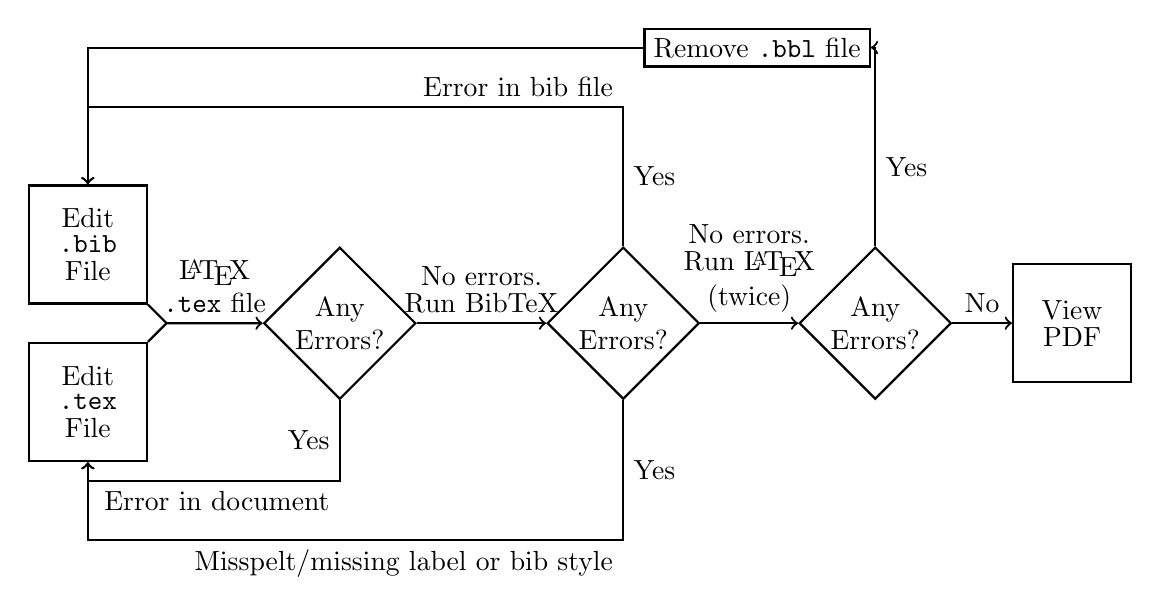
\begin{tikzpicture}[thick]
      \begin{scope}[minimum width=1.5cm,minimum height=1.5cm,inner sep=.1em]
        \path (0,0) node[draw] (edit) {\shortstack{Edit\\\texttt{.tex}\\File}};
        \path (0,2) node[draw] (editbib) {\shortstack{Edit\\\texttt{.bib}\\File}};
        \path (3.2,1) node[draw,diamond] (errors) 
          {\shortstack{Any\\Errors?}};
        \path (6.8,1) node[draw,diamond] (bibtexerrors)
          {\shortstack{Any\\Errors?}};
        \path (10,1) node[draw,diamond] (errors2)
          {\shortstack{Any\\Errors?}};
        \path (12.5,1) node[draw] (pdf) {\shortstack{View\\PDF}};
      \end{scope}
      \path (8.5,4.5) node[draw,rectangle] (rmbbl) {Remove \texttt{.bbl} file};
      \draw[->] (edit) -- (1,1) -- (errors) node[midway,above] 
        {\shortstack{\LaTeX{}\\\texttt{.tex} file}};
      \draw (editbib) -- (1,1);
      \draw[->] (errors) -- ++(0,-2) node[midway,left] {Yes}
        -| (edit) node[pos=0,below,anchor=north east] 
          {Error in document};
      \draw[->] (errors) -- (bibtexerrors)
        node[midway,above] {\shortstack{No errors.\\Run \BibTeX{}}};
      \draw[->] (bibtexerrors) -- ++(0,-2.75)
        node[midway,right] {Yes} -| (edit) 
        node[pos=0,below,anchor=north east] 
          {Misspelt/missing label or bib style};
      \draw[->] (bibtexerrors) -- ++(0,2.75) node[midway,right] 
        {Yes} -| (editbib) node[pos=0,above,anchor=south east] 
        {Error in bib file};
      \draw[->] (bibtexerrors) -- (errors2) node[midway,above] 
        {\shortstack{No errors.\\Run \LaTeX{}\\(twice)}};
      \draw[->] (errors2) |- (rmbbl) node[pos=0.2,right] {Yes};
      \draw[->] (rmbbl) -| (editbib);
      \draw[->] (errors2) -- (pdf) node[midway,above] {No};
    \end{tikzpicture}%
  }

\end{frame}

\begin{frame}[fragile]{The \BibTeX{} file}{A basic article}

  \begin{example}
    \begin{semiverbatim}
\alert<2>{@book}\{\alert<3>{lamport94},
   author    = "Leslie Lamport",
   title     = 
     "\alert<4>{\{\\LaTeX\{\}\}}: a document preparation system",
   edition   = "2nd",
   publisher = "Addison-{}-Wesley",
   year      = \alert<5>{1994},
\}
    \end{semiverbatim}
  \end{example}

\end{frame}

\begin{frame}[fragile]{The \BibTeX{} file}{Multiple authors}

  \begin{example}
    \begin{semiverbatim}
@inproceedings\{smith05,
  author    = "Smith, Jr, John \alert<2>{and} Jane Lucy Doe
   \alert<2>{and} Other, Andrew N. \alert<2>{and} de Vere, Jo",
  title     = "An example article",
  booktitle = "Proceedings of the Imaginary Society",
  month     = JAN
  year      = 2005
\}
    \end{semiverbatim}
  \end{example}

\end{frame}

\begin{frame}[fragile]{Citations in \LaTeX{}}

  \begin{itemize}
    \item The \LaTeX{} kernel is limited for citations;
    \item The \pkg{natbib} package is much more powerful;
    \item A new approach is provided by \pkg{biblatex}.
  \end{itemize}

\end{frame}

\begin{frame}{Citations using \pkg{natbib}}

  \begin{block}{Textual citations}
    \vspace*{0.5 em}
    \begin{tabular}{l@{\ $\Rightarrow$\ }l}
      \multicolumn{2}{l}{%
        \cs{citet}\oarg{\meta{note}}\marg{\meta{key}}%
      } \\[0.5em]
      \cs{citet}\marg{lamport1994} & Lamport (1994) \\
      \cs{citet}\oarg{p.\textasciitilde34}\marg{lamport1994} &
        Lamport (1994, p.~34) \\
    \end{tabular}
  \end{block}
  
  \begin{block}{Parenthetical citations}
    \vspace*{0.5 em}
    \begin{tabular}{l@{\ $\Rightarrow$\ }l}
      \multicolumn{2}{l}{%
        \cs{citep}\oarg{\meta{prenote}}\oarg{\meta{postnote}}%
        \marg{\meta{key}}%
      }  \\[0.5em]
      \cs{citep}\marg{lamport94} & (Lamport, 1994)\\
      \cs{citep}\oarg{p.\textasciitilde34}\marg{lamport94} 
        & (Lamport, 1994, p.~34)\\
      \cs{citep}\oarg{see}\oarg{}\marg{lamport94} & (see Lamport, 1994)
    \end{tabular}
  \end{block}
  
\end{frame}

\begin{exercise}
  Create a file called \texttt{myrefs.bib} that contains the
  following:
  \verbatiminput{examples/myrefs.bib}

  Then create a file called, say, \texttt{example5.tex} that contains
  the following:
  \verbatiminput{examples/example6.tex}

  If you are using a terminal or command prompt, you will need to use
  the following commands:
  \begin{verbatim}
    pdflatex example5
    bibtex example5
    pdflatex example5
    pdflatex example5
  \end{verbatim}

  There are various options you can pass to the \pkg{natbib} package
  that affects the formatting. For example:
  \begin{verbatim}
    \usepackage[numbers,sort&compress]{natbib}
  \end{verbatim}
  Try experimenting with some of these options: \texttt{round},
  \texttt{curly} and \texttt{numbers}. With the \texttt{numbers}
  option, you can also use: \texttt{super}, \texttt{sort}
  and \texttt{sort\&compress}.
\end{exercise}

\section{Long documents}

\begin{frame}{Working with long documents}

  \begin{itemize}
    \item Long documents are best split into parts;
    \item \cs{input} places the material loaded \enquote{here};
    \item \cs{include} is used for separate chapters:\\ it always starts
      a new page;
    \item Using \cs{include} allows you to \cs{includeonly}\\
      selected chapters;
    \item Use \cs{includeonly} in the preamble.
  \end{itemize}
  
\end{frame}

\begin{exercise}

  Create a master file
  \verbatiminput{examples/example7.tex}
  along with the three chapters, each of which can be as simple as
  \begin{verbatim}
    \chapter{A demo}
    \lipsum
  \end{verbatim}
  Experiment with this basic structure, and using \cs{includeonly} to
  use only some of the files.

\end{exercise}

\tutornote{Finish exercise at 15:45 and break for coffee}

\section{Further information}

\begin{frame}{Getting help}

  \begin{itemize}
    \item \url{www.tex.ac.uk/faq};
    \item \url{wwww.latex-community.org};
    \item \url{tex.stackexchange.com};
    \item \url{theoval.cmp.uea.ac.uk/~nlct/latex/};
    \item \url{detexify.kirelabs.org/}.
  \end{itemize}

\end{frame}

\begin{frame}{Reading}

  \begin{itemize}
    \item \emph{Not So Short Introduction to \LaTeXe{}}, Oetiker;
    \item \emph{A Guide to \LaTeX{}}, Kopka and Daly;
    \item \emph{\LaTeX{} Beginners Guide}, Kottwitz;
    \item \emph{\LaTeX{} and Friends}, van Dongen.
  \end{itemize}

\end{frame}

\tutornote{Time allowing, simple \textsf{hyperref} demo is good here}

\end{document}

